\section{Bibliotheken}
\begin{table*}
\centering

% Diese Tabelle wurde mühsam angeordnet. Bitte nicht umbrechen, sondern scrollen!
%~ \newcommand{\bibKIP}{}
\begin{tabular}{lll@{ -- }l@{\quad}r@{ -- }l@{ Uhr}}
\toprule
Name                                    & Adresse                                                                                                                       & \multicolumn{4}{l}{"Offnungszeiten}    \\
\midrule
\multirow{5}{*}{\gls{UB} (Ausleihe)}    & \multirow{2}{*}{\href{http://www.openstreetmap.org/?mlat=49.40966&mlon=8.70594&zoom=17&layers=M}{Plöck 107-109 (Altstadt)}}   & Mo & Fr                    & \ubAltAusMoFr \\
                                        &                                                                                                                               & \multicolumn{2}{l}{Sa}     & \ubAltAusSa \\[-0.7\defaultaddspace]
                                        & \multicolumn{1}{c}{}                                                                                                                                                \\[-0.7\defaultaddspace]
                                        & \multirow{2}{*}{\href{http://www.openstreetmap.org/?mlat=49.41767&mlon=8.66836&zoom=17&layers=M}{INF 368, 3. Stock (Feld)}}   & Mo & Fr                    & \ubFeldAusMoFr \\
                                        &                                                                                                                               & \multicolumn{2}{l}{Sa}     & \ubFeldAusSa \\
\cmidrule{1-6}
\multirow{5}{*}{\gls{UB} (Lesesaal)}    & \multirow{2}{*}{\href{http://www.openstreetmap.org/?mlat=49.40966&mlon=8.70594&zoom=17&layers=M}{Plöck 107-109 (Altstadt)}}   & Mo & Fr                    & \ubAltLesMoFr \\
                                        &                                                                                                                               & Sa & So                    & \ubAltLesSa \\[-0.7\defaultaddspace]
                                        & \multicolumn{1}{c}{}                                                                                                                                                \\[-0.7\defaultaddspace]
                                        & \multirow{2}{*}{\href{http://www.openstreetmap.org/?mlat=49.41767&mlon=8.66836&zoom=17&layers=M}{INF 368 (Feld)}}             & Mo & Fr                    & \ubFeldAusMoFr \\
                                        &                                                                                                                               & Sa & So                    & \ubFeldAusSa \\
\cmidrule{1-6}
\multirow{2}{*}{Mathematikon}           & \multirow{2}{*}{\href{http://www.openstreetmap.org/?mlat=49.41730&mlon=8.67580\#map=17/49.41730/8.67580}{INF 205}}            & Mo & Fr                    & \mathekonMoFr \\
                                        &                                                                                                                               & \multicolumn{2}{l}{Sa}     & \mathekonSa\\
\cmidrule{1-6}
\multirow{2}{*}{Physik}                 & \multirow{2}{*}{\href{http://www.openstreetmap.org/?mlat=49.41479&mlon=8.69686&zoom=17&layers=M}{Philosophenweg 16}}          & Mo & Fr                    & \physikMoFr \\
                                        &                                                                                                                               & \multicolumn{2}{l}{}       & \physikSa \\
\cmidrule{1-6}
\multirow{3}{*}{Stadtbücherei}          & \multirow{3}{*}{\href{http://www.openstreetmap.org/?mlat=49.40638&mlon=8.6866&zoom=17&layers=M}{Poststraße 15}}               & Di & Fr                    & 10   & 20 \\
                                        &                                                                                                                               & \multicolumn{2}{l}{Sa}     & 10   & 16 \\
                                        &                                                                                                                               & \multicolumn{4}{l}{Montags geschlossen!}\\
\cmidrule{1-6}
\multirow{2}{*}{Studibücherei}          & \multirow{2}{*}{\href{http://www.openstreetmap.org/?mlat=49.41051&mlon=8.70518&zoom=17&layers=M}{Grabengasse 14}}               & Mo & Do                    & 11   & 17 \\
                                        &                                                                                                                            & \multicolumn{2}{l}{Fr}     & 11   & 14 \\
\cmidrule{1-6}
\multirow{2}{*}{Hinweis:}               & \multicolumn{4}{c}{\textbf{Während der vorlesungsfreien Zeit gelten veränderte Zeiten.}} \\                  
                                        & \multicolumn{4}{c}{\textbf{Bitte schaut dafür auf der jeweiligen Website nach.}} \\

\bottomrule
\end{tabular}

\end{table*}

Fachliteratur ist meistens unglaublich teuer. Um den totalen Ruin der Studierenden zu vermeiden, hat jede Universität Bibliotheken. In Heidelberg ist die \gls{UB} dreigeteilt, und zwar entsprechend der Dreiteilung der Universität. Die für euch wahrscheinlich interessanteste Literatur über Mathe, Informatik und Physik befindet sich in der Zweigstelle \gls{INF}~368, 3.~Stock.

\begin{figure*}[t]
\centering
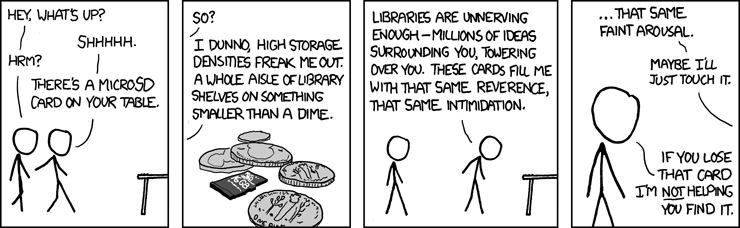
\includegraphics[width=\textwidth]{bilder/library.png}
\end{figure*}


Neben Physik-, Informatik- und Mathebüchern können hier auch medizinische Literatur und Bücher für alle anderen Fakultäten, die im Neuenheimer Feld untergebracht sind, ausgeliehen werden. Im Hauptsitz der \gls{UB} an der Peterskirche, Plöck~107-109, und der Campus-Bibliothek in Bergheim hingegen findet sich geisteswissenschaftliche Literatur sowie zahlreiche Jura- und VWL- Bücher. Bedingt durch diese Dreiteilung wurde in Heidelberg sehr früh ein Computersystem („\gls{HEIDI}“\footnote{\url{http://katalog.ub.uni-heidelberg.de}}) in der UB eingeführt. Mit Hilfe von Heidi und eurer Uni-ID, die auf eurem Studiausweis steht, kann dort die gängige Fachliteratur ausgeliehen werden. Übers Internet lässt sich auch direkt nach Büchern suchen, außerdem können ausgeliehene Bücher online verlängert werden -- das kann einem durchaus den ein oder anderen Euro sparen, die Mahngebühren bei überzogenen Fristen sind nämlich empfindlich teuer. Viele Bücher lassen sich auch als PDFs downloaden oder wenigstens als E-Book online abrufen. Zu Semesterbeginn finden in der UB Einführungskurse in Heidi statt, die jedoch nur bedingt sinnvoll sind, weil das System sehr übersichtlich und intuitiv aufgebaut ist und sich größtenteils selbsterklärend bedienen lässt.

So ist es bspw. möglich über die Suche festzustellen, ob ein Buch als E-Book aufrufbar ist. Der jeweilige Sucheintrag enthält dann links-unten einen „Online-Ressource“-Hinweis. Auf der jeweiligen Seite des Buches findet sich dann links-oben ein Link „online aufrufen“, der zu der E-Book-Version führt, nachdem du „Universität Heidelberg“ angewählt und dich mit deiner Uni-ID angemeldet hast. 

Mittels Heidi lassen sich auch Gruppenarbeitsräume in den Bibliotheken kostenfrei reservieren, was insbesondere praktisch für das Zettellösen in Gruppenarbeit am Wochenende ist.

Wer weiterführende spezielle Fachliteratur sucht, muss sich an die Bereichsbibliotheken der einzelnen Fakultäten richten, deren Bestände ebenfalls in \gls{HEIDI} erfasst sind. Für Mathe- und Informatik-Literatur befindet sich die Bereichsbibliothek im Gebäude \gls{INF}~205 (im Erdgeschoss auf der Ostseite). Weitere Informationen und Öffnungszeiten finden sich auf der Webseite der Bereichsbibliothek.\footnote{\url{https://www.mathinf.uni-heidelberg.de/bib}} Spezielle Physikbücher findet man an den Standorten der Bereichsbibliothek Physik und Astronomie (BPA), welche ihren zentralen Sitz am Philosophenweg~16 hat.\footnote{\url{http://www.ub.uni-heidelberg.de/dezentral/bpa/standorte.html}} Auch wenn die Lage etwas abschreckend wirken mag, lohnt sich ein Besuch, alleine wegen des Gebäudes. Die Bibliothekarinnen freuen sich sehr über studentischen Besuch. Die Bereichsbibliothek der Physik führt auch weitere Standorte in einzelnen Instituten, hier kommt man jedoch erst nach Vereinbarung rein.
Bei den Bereichsbibliotheken handelt es sich um Präsenzbibliotheken. Das bedeutet, dass man Bücher und Zeitschriften vor Ort kopieren, aber nicht ausleihen, darf. Für die Ausleihe spezieller Werke können jedoch auch Ausnahmen gemacht werden, z.B. im Falle eines für eine Abschlussarbeit notwendiges Buches, welches nur in der Bereichsbibliothek geführt wird.
Wenn ein Buch in der UB komplett ausgeliehen ist, dann lohnt es sich manchmal auch, zur Stadtbücherei in der Poststraße zu gehen. Zum Anmelden braucht man nur einen Personalausweis. Die Ausleihe ist allerdings nicht kostenlos (\EUR{10}/Jahr). Weitere Information kannst du auch direkt bei der Stadtbücherei einholen.\footnote{\url{https://www.heidelberg-stadtbuecherei.de}}

Solltest du Werke in physischer oder digitaler Form vermissen, so kannst du über das Anschaffungsvorschlagsformular der Universitätsbibliothek\footnote{\url{https://www.ub.uni-heidelberg.de/allg/benutzung/bereiche/vorschlag.html}} Vorschläge einbringen. Für physiknahe Werke kannst du dich auch an uns als Fachschaft wenden, da in der Physik ein Bibliotheksausschuss existiert, in welchem auch eine studentische Vertreterin, genau für solche Zwecke, sitzt.
 
Das Studierendenwerk bietet zusätzlich noch die Studierendenbibliothek\footnote{\url{http://www.studentenwerk.uni-heidelberg.de/de/studibuecherei}}, welche neben geistenswissenschaftlicher Fachliteratur auch insbesondere Welt-, Kriminial- und Unterhaltungsliteratur in ihrem Bestand hat. Die Studierendenbibliothek, wie auch die Stadtbücherei laden dazu ein, neben der ganzen Studiererei auch einfach mal abzuschalten und zu schmökern.
